\documentclass[tikz,border=10pt]{standalone}
\usepackage{tikz}
\usetikzlibrary{positioning}

\begin{document}

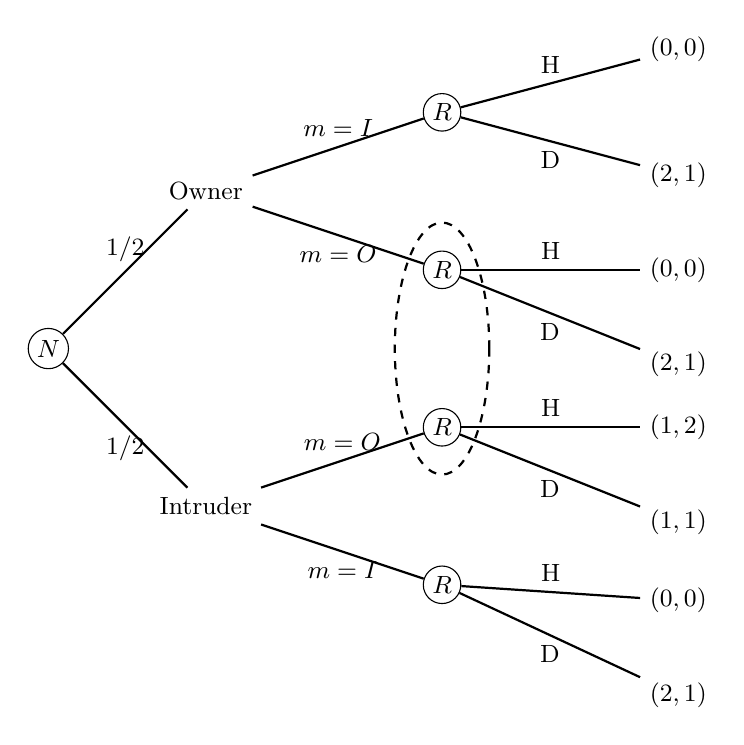
\begin{tikzpicture}[
    font=\small,
    decision/.style={circle,draw,inner sep=1.5pt},
    chance/.style={circle,draw,inner sep=1.5pt},
    line/.style={thick},
    infoset/.style={thick,dashed}
]

% === Nature ===
\node[chance] (N) at (0,0) {$N$};

% === Types ===
\node (O) at (2,2) {Owner};
\node (I) at (2,-2) {Intruder};

\draw[line] (N) -- node[above] {$1/2$} (O);
\draw[line] (N) -- node[below] {$1/2$} (I);

% === Receiver nodes ===
\node[decision] (RO_I) at (5,3) {$R$};    % Owner → m=I
\node[decision] (RO_O) at (5,1) {$R$};    % Owner → m=O
\node[decision] (RI_O) at (5,-1) {$R$};   % Intruder → m=O
\node[decision] (RI_I) at (5,-3) {$R$};   % Intruder → m=I

% === Messages ===
\draw[line] (O) -- node[above] {$m=I$} (RO_I);
\draw[line] (O) -- node[below] {$m=O$} (RO_O);
\draw[line] (I) -- node[above] {$m=O$} (RI_O);
\draw[line] (I) -- node[below] {$m=I$} (RI_I);

% === Information set for m=O ===
\draw[infoset] (5,0) ellipse (0.6 and 1.6);

% === Terminal nodes (симметрично и с равным интервалом) ===
\node (S1) at (8,3.8) {$(0,0)$};   % Owner→m=I, H
\node (S2) at (8,2.2) {$(2,1)$};   % Owner→m=I, D
\node (S3) at (8,1.0) {$(0,0)$};   % Owner→m=O, H
\node (S4) at (8,-0.2) {$(2,1)$};  % Owner→m=O, D
\node (S5) at (8,-1.0) {$(1,2)$};  % Intruder→m=O, H
\node (S6) at (8,-2.2) {$(1,1)$};  % Intruder→m=O, D
\node (S7) at (8,-3.2) {$(0,0)$};  % Intruder→m=I, H
\node (S8) at (8,-4.4) {$(2,1)$};  % Intruder→m=I, D

% === Connect Receiver nodes to terminal payoffs ===
\draw[line] (RO_I) -- node[above] {H} (S1);
\draw[line] (RO_I) -- node[below] {D} (S2);

\draw[line] (RO_O) -- node[above] {H} (S3);
\draw[line] (RO_O) -- node[below] {D} (S4);

\draw[line] (RI_O) -- node[above] {H} (S5);
\draw[line] (RI_O) -- node[below] {D} (S6);

\draw[line] (RI_I) -- node[above] {H} (S7);
\draw[line] (RI_I) -- node[below] {D} (S8);

% === Label ===
% \node at (4.5,-5.5) {\textbf{Cheap talk: Bourgeois not ESS}};

\end{tikzpicture}

\end{document}
